% !TEX program = xelatex
\documentclass[11pt]{article}
\usepackage{kotex}
\usepackage{booktabs}
\usepackage{siunitx}
\usepackage{pgfplots}
\usepackage{geometry}
\geometry{margin=1in}
\pgfplotsset{compat=1.18}
\sisetup{round-mode=places,round-precision=2}

\title{RPL/BRPL 실험 결과 요약}
\author{}
\date{}

\begin{document}
\maketitle

\section*{요약}
본 문서는 \texttt{results/summary.csv}를 기반으로 한 실험 결과 요약이다.
붕괴 시점 탐지는 아래 기준을 사용했다.

\section*{붕괴 기준}
\begin{itemize}
  \item 패킷 전달률(PDR): $ \mathrm{PDR} = \frac{\mathrm{rx\_count}}{\mathrm{tx\_expected}} $
  \item 붕괴 조건: $\mathrm{PDR} < 0.9$ 또는 $\mathrm{rx\_count} \le 0$
  \item 제어 오버헤드(초당): $ \mathrm{overhead\_per\_s} = \frac{\mathrm{dio\_count}+\mathrm{dao\_count}}{\mathrm{duration\_s}} $
\end{itemize}

\section*{모드/스테이지별 요약 통계}
\begin{table}[h]
\centering
\caption{모드/스테이지별 평균/중앙값 요약}
\begin{tabular}{llrrrrr}
\toprule
Mode & Stage & PDR & Avg Delay(ms) & P95 Delay(ms) & Overhead/s & Runs \\
\midrule
brpl & stage1 & 0.00 & 0.00 & 0.00 & 2.67 & 69 \\
brpl & stage2 & 0.00 & 0.00 & 0.00 & 2.74 & 72 \\
brpl & stage3 & 0.00 & 0.00 & 0.00 & 3.15 & 12 \\
rpl-classic & stage1 & 1.00 & 382.21 & 574.57 & 10.59 & 121 \\
rpl-classic & stage2 & 1.00 & 456.99 & 943.87 & 24.38 & 173 \\
rpl-classic & stage3 & 1.00 & 418.27 & 690.10 & 24.03 & 12 \\
\bottomrule
\end{tabular}
\end{table}

\section*{붕괴 시점(최초 발생 조건)}
\begin{table}[h]
\centering
\caption{Stage별 붕괴 조건(최초 발생 기준)}
\begin{tabular}{llrrrr}
\toprule
Mode & Stage & N & Success Ratio & Interference Ratio & Send Interval(s) \\
\midrule
brpl & stage1 & 5 & 1.00 & 1.00 & 10 \\
brpl & stage2 & 50 & 1.00 & 0.85--1.00 & 10 \\
brpl & stage3 & 50 & 1.00 & 1.00 & 2 \\
rpl-classic & stage1--3 & \multicolumn{4}{l}{붕괴 조건 미검출} \\
\bottomrule
\end{tabular}
\end{table}

\section*{Stage 2/3 상세 붕괴 조건}
\subsection*{Stage 2}
\begin{table}[h]
\centering
\caption{Stage 2 붕괴 조건 상세}
\begin{tabular}{lrrrrr}
\toprule
Mode & N & Success Ratio & Interference Ratio & PDR & Runs \\
\midrule
brpl & 50 & 1.00 & 0.85 & 0.00 & 3 \\
brpl & 50 & 1.00 & 0.90 & 0.00 & 3 \\
brpl & 50 & 1.00 & 0.95 & 0.00 & 3 \\
brpl & 50 & 1.00 & 1.00 & 0.00 & 3 \\
\bottomrule
\end{tabular}
\end{table}

\subsection*{Stage 3}
\begin{table}[h]
\centering
\caption{Stage 3 붕괴 조건 상세}
\begin{tabular}{lrrrrrr}
\toprule
Mode & N & Success Ratio & Interference Ratio & Send Interval(s) & PDR & Runs \\
\midrule
brpl & 50 & 1.00 & 1.00 & 2 & 0.00 & 3 \\
\bottomrule
\end{tabular}
\end{table}

\section*{시각화}
\subsection*{PDR 비교}
\begin{figure}[h]
\centering
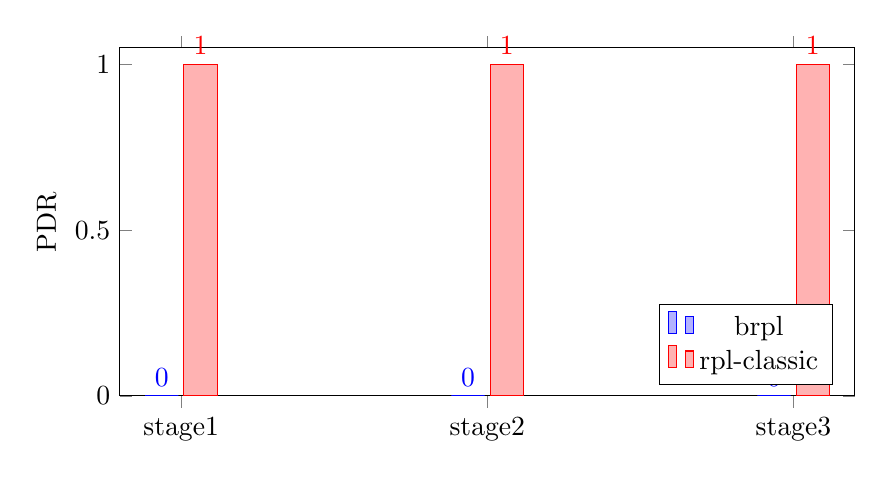
\begin{tikzpicture}
\begin{axis}[
  ybar,
  bar width=12pt,
  width=0.9\textwidth,
  height=6cm,
  ymin=0, ymax=1.05,
  ylabel={PDR},
  symbolic x coords={stage1,stage2,stage3},
  xtick=data,
  legend pos=south east,
  nodes near coords,
  nodes near coords align={vertical},
]
\addplot coordinates {(stage1,0.00) (stage2,0.00) (stage3,0.00)};
\addplot coordinates {(stage1,1.00) (stage2,1.00) (stage3,1.00)};
\legend{brpl,rpl-classic}
\end{axis}
\end{tikzpicture}
\caption{Stage별 평균 PDR 비교}
\end{figure}

\subsection*{제어 오버헤드 비교}
\begin{figure}[h]
\centering
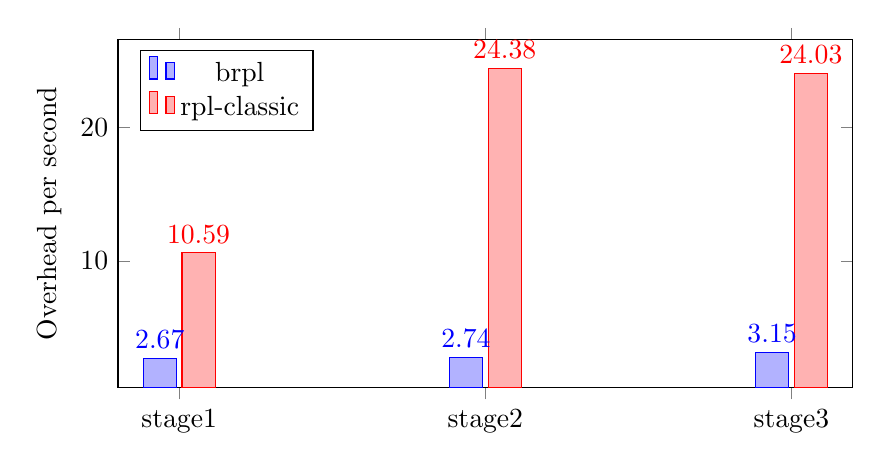
\begin{tikzpicture}
\begin{axis}[
  ybar,
  bar width=12pt,
  width=0.9\textwidth,
  height=6cm,
  ylabel={Overhead per second},
  symbolic x coords={stage1,stage2,stage3},
  xtick=data,
  legend pos=north west,
  nodes near coords,
  nodes near coords align={vertical},
]
\addplot coordinates {(stage1,2.67) (stage2,2.74) (stage3,3.15)};
\addplot coordinates {(stage1,10.59) (stage2,24.38) (stage3,24.03)};
\legend{brpl,rpl-classic}
\end{axis}
\end{tikzpicture}
\caption{Stage별 평균 제어 오버헤드 비교}
\end{figure}

\section*{해석}
\begin{itemize}
  \item brpl은 모든 stage에서 PDR이 0으로 집계되어 초기부터 붕괴로 판정되었다.
  \item rpl-classic은 모든 stage에서 PDR이 1.0으로 유지되어 붕괴 조건이 관측되지 않았다.
  \item brpl 결과는 정상 송신/수신이 이루어졌는지 추가 점검이 필요하다.
\end{itemize}

\end{document}
